% 导体

\pentry{电场的高斯定理\upref{EGauss}}

\subsection{导体的电荷分布}
带净电荷的导体有一个显著的性质就是净电荷只分布于其表面, 且表面的电荷分布使得导体内部电场强度为零. 我们可以用高斯定理来证明这个性质. 假设导体达到了静电平衡, 则其内部的电荷分布稳定且没有任何(宏观上的)的电流. 如果导体内部存在任何净电荷, 在净电荷周围做一个高斯面, 则高斯面上必然会有电场, 进而产生电流, 这就违背了静电平衡的假设.

由于内部电场强度为零, 导体在静电平衡时处处电势相等, 是一个\bb{等势体}.


blablabla...

\begin{exam}{匀强电场中的球形导体}
匀强电场 $\vec E_0$ 中有一个半径为 $R$ 的导体球处于静电平衡, 求导体球表面的电荷分布.

我们取电场的方向为球坐标的极轴, 由问题的对称性, 电荷分布关于极轴对称, 所以电荷面密度可以表示为 $\sigma(\theta)$. 我们现在需要寻找一个 $\sigma(\theta)$ 使得表面电荷在导体球内部可以产生与外电场 $\vec E_0$ 等大反向的匀强电场.

\begin{figure}[ht]
\centering
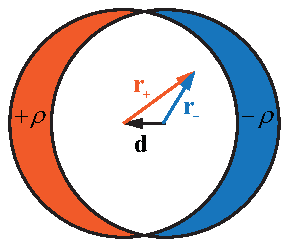
\includegraphics[width=5cm]{./figures/Cndctr1.pdf}
\caption{两个重叠的均匀带电导体球} \label{Cndctr_fig1}
\end{figure}

这里介绍一种巧妙的办法, 我们先来看以下一个模型. 先假设不存在外电场, 令两个电荷密度分别为 $\pm\rho$ 的均匀带电球在极轴方向错开距离 $d$ ($d < R$) 两球重合的部分正负电荷叠加, 净电荷为零. 令 $\pm\rho$ 的球心指向空间中某点的矢量分别为 $\vec r_\pm$, 根据\autoref{EGauss_exe3}\upref{EGauss} 中的结论, 我们知道两球产生的电场分别为
\begin{equation}
\vec E_\pm = \frac{\rho}{3\epsilon_0}\vec r_\pm
\end{equation}
令 $-\rho$ 的球心指向 $+\rho$ 球心的矢量为 $\vec d$, 有 $\vec r_+ - \vec r_- = -\vec d$, 所以两球重合区域中任意一点的总电场为
\begin{equation}
\vec E = \vec E_+ + \vec E_- = \frac{\rho}{3\epsilon_0}(\vec r_+ - \vec r_-) = -\frac{\rho}{3\epsilon_0}\vec d
\end{equation}
这是一个匀强电场, 恰好符合我们的要求. 现在就可以令 $\vec d\to \vec 0$, 然后计算电荷面密度, 面密度与厚度 $h$ 成正比. 由\autoref{Cndctr_fig2} 可得 $h = d\cos\theta$.

\begin{figure}[ht]
\centering
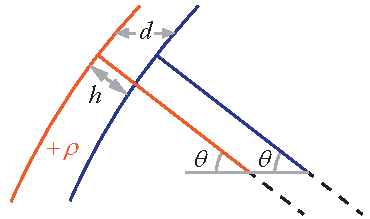
\includegraphics[width=6.5cm]{./figures/Cndctr2.pdf}
\caption{两个重叠的均匀带电导体球 $\theta$} \label{Cndctr_fig2}
\end{figure}

所以面密度就是 $\sigma(\theta) = \rho h = \rho d\cos\theta = 3\epsilon_0 E \cos\theta$. 若 $\vec E$ 要与外电场 $\vec E_0$ 抵消, 令 $E = E_0$ 可得
\begin{equation}
\sigma(\theta) = 3\epsilon_0 E_0 \cos\theta
\end{equation}
\end{exam}

